\section{Basics of networking commands}
\subsection{Aim}
To get started with the basics of networking configuration files and networking
commands in Linux.
\subsection{Networking Commands}
\subsubsection{ifconfig}
ifconfig is used to configure network interfaces. It has features 
for configuring, controlling and querying TCP/IP network interface paramaters.
\linebreak[2]


Syntax:
\begin{lstlisting}
ifconfig [-AaC] [interface] [address_family] [address [dest_address]] 
	[parameters]
\end{lstlisting}

\begin{center}
	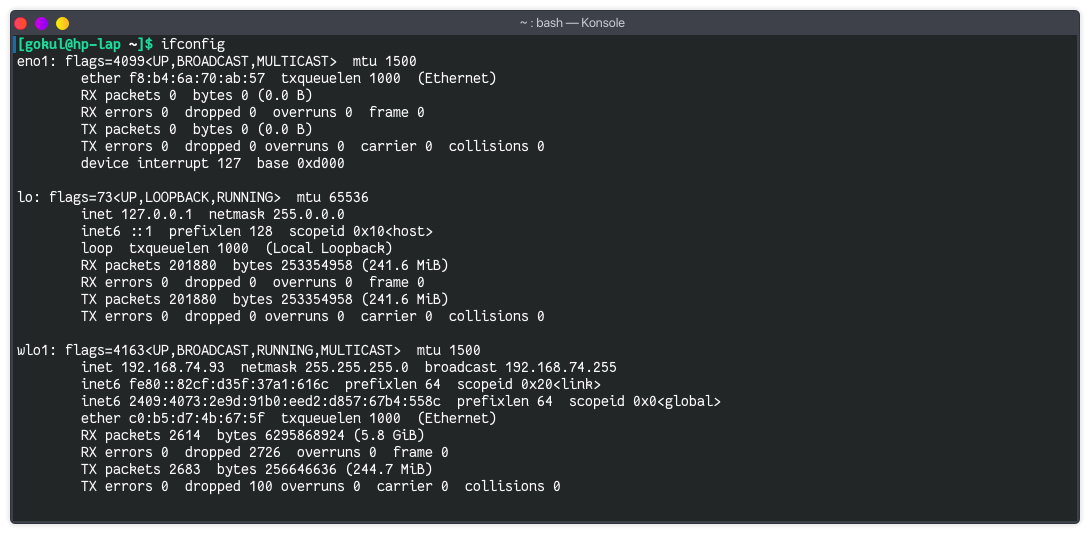
\includegraphics[width=0.90\textwidth]{img/p1/ss1.png}
\end{center}


\subsubsection{ping}
Packet Internet Groper (PING) is used to check network connectivity 
between host and server/host. The input for the command is the IP 
address or the URL of the host to check connectivity of. 
It sends a data packet to the specified address with the message "PING"
and recieves response from the server/host. The time for this
recorded and displayed as latency. 

PING uses Internet Control Message Protocol (ICMP) to send an ICMP echo message
to the specified host and if the host is available it responds with ICMP reply message.
\linebreak[2]

Syntax:
\begin{lstlisting}
ping [-aAbBdDfhLnOqrRUvV6] [-c count] [-F flowlabel] [-i interval] 
	[-I interface] [-l preload] [-m mark] [-M pmtudisc_option] 
	[-N nodeinfo_option] [-w deadline] [-W timeout] [-p pattern] 
	[-Q tos] [-s packetsize] [-S sndbuf] [-t ttl] 
	[-T timestamp option] [hop ...] 
	destination
\end{lstlisting}

\begin{center}
	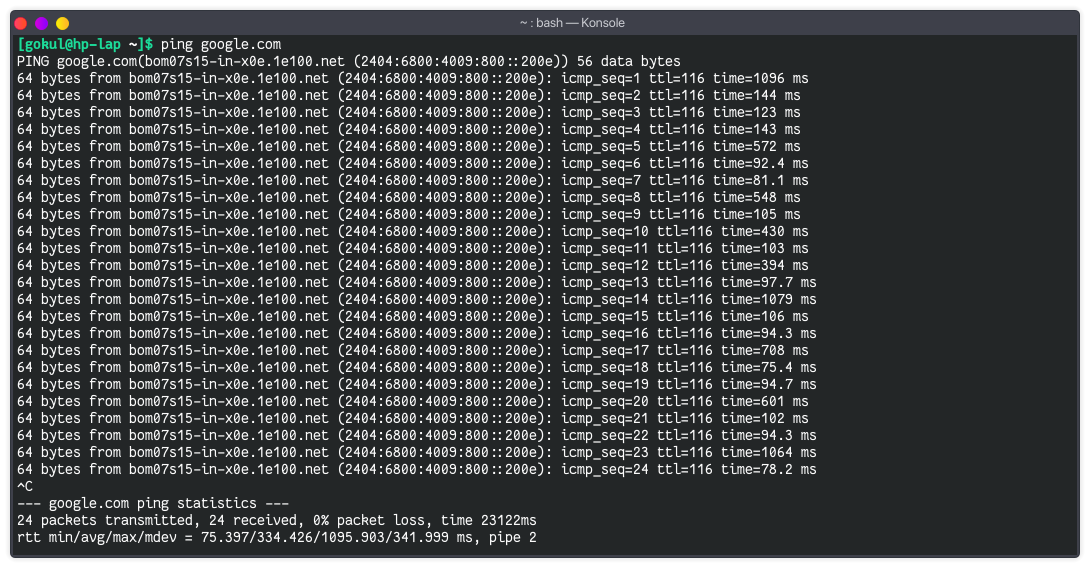
\includegraphics[width=0.90\textwidth]{img/p1/ss2.png}
\end{center}


\subsubsection{traceroute}
traceroute command shows the path to reach a network resource. It is also used to measure
transit delays of packet across Internet Protocol network.
\linebreak[2]

Syntax:
\begin{lstlisting}
traceroute [-FIldnrv] [-f 1st_ttl] [-m max_ttl] [-p port#] [-q nqueries]
	[-s src_addr] [-t tos] [-w wait] [-g gateway] [-i iface] 
	[-z pausemsecs] HOST [data size]
\end{lstlisting}

\begin{center}
	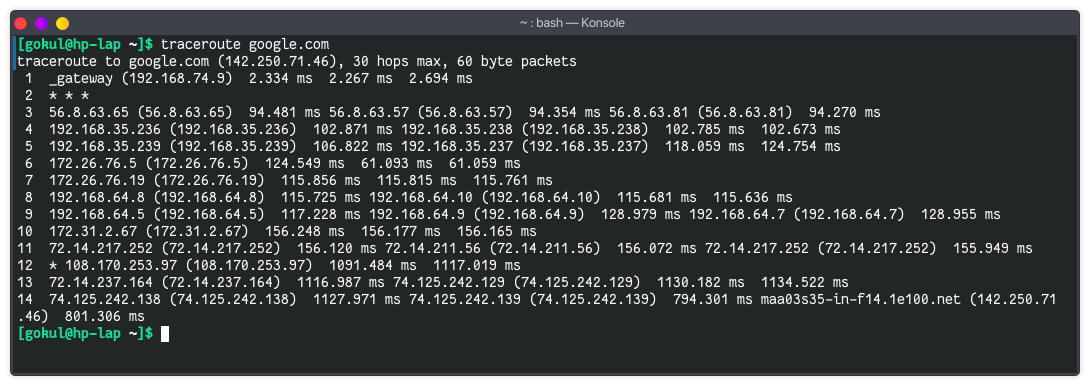
\includegraphics[width=0.90\textwidth]{img/p1/ss3.png}
\end{center}


\subsubsection{netstat}
netstat is a command-line network utility that displays network connections 
for Transmission Control Protocol, routing tables, and a number of network interface 
and network protocol statistics.
\linebreak[2]

Syntax:
\begin{lstlisting}
netstat [address_family_options] [--tcp|-t] [--udp|-u] [--raw|-w] 
	[--listening|-l] [--all|-a] [--numeric|-n] 
	[--numeric-hosts][--numeric-ports][--numeric-ports] 
	[--symbolic|-N] [--extend|-e[--extend|-e]] [--timers|-o] 
	[--program|-p] [--verbose|-v] [--continuous|-c] [delay]
\end{lstlisting}

\begin{center}
	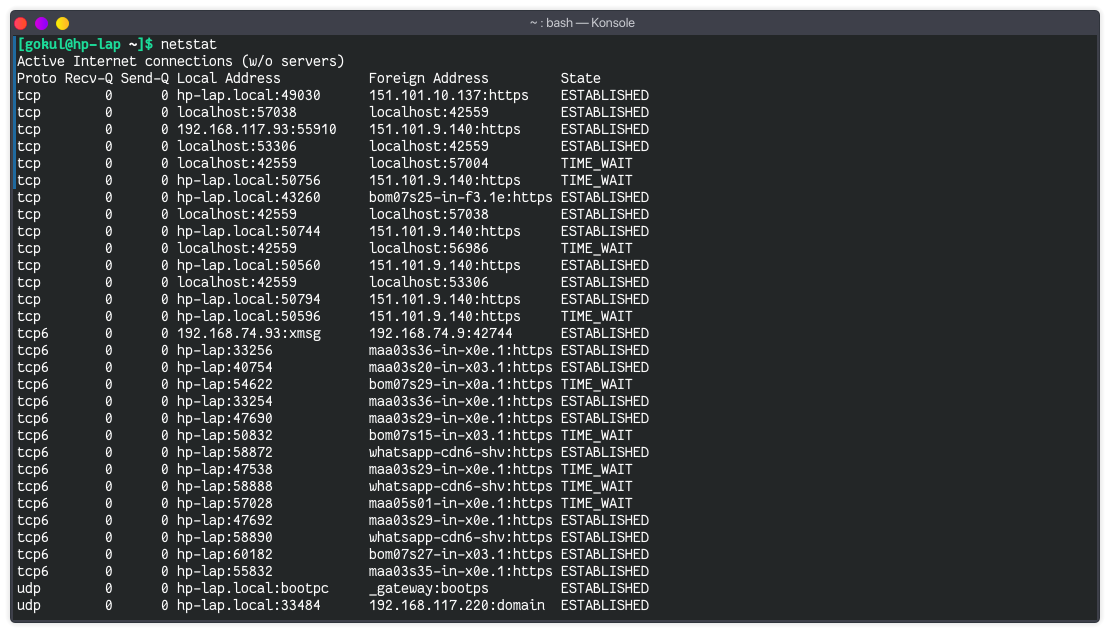
\includegraphics[width=0.90\textwidth]{img/p1/ss4.png}
\end{center}


\subsubsection{nslookup}
nslookup is a network administration command-line tool for querying the 
Domain Name System to obtain domain name or IP address mapping, or other DNS records.
\linebreak[2]

Syntax:
\begin{lstlisting}
nslookup [HOST] [SERVER]
\end{lstlisting}

\begin{center}
	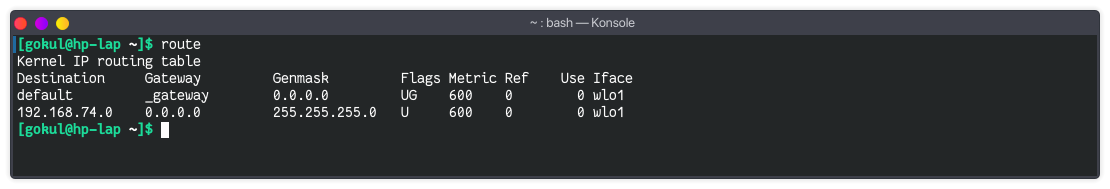
\includegraphics[width=0.90\textwidth]{img/p1/ss5.png}
\end{center}


\subsubsection{route}
Route manipulates the kernel's IP routing tables. Its primary use is to set up static routes 
to specific hosts or networks via an interface after it has been configured with the ifconfig.
When the add or del options are used, route modifies the routing tables. Without these options, 
route displays the current contents of the routing tables
\linebreak[2]

Syntax:
\begin{lstlisting}
route [-v] [-A family] add [-net|-host] target [netmask Nm] [gw Gw] 
	[metric N] [mss M] [window W] [irtt I] [reject] [mod] [dyn] 
	[reinstate] [[dev] If]
\end{lstlisting}

\begin{center}
	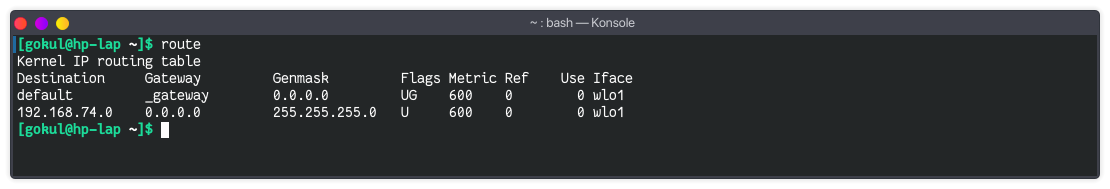
\includegraphics[width=0.90\textwidth]{img/p1/ss6.png}
\end{center}


\subsubsection{dig}
dig is a flexible tool for interrogating DNS name servers. It performs DNS lookups and displays the answers 
that are returned from the name server(s) that were queried. Most DNS administrators use dig to troubleshoot 
DNS problems because of its flexibility, ease of use, and clarity of output.
Unless it is told to query a specific name server, dig tries each of the servers listed in /etc/resolv.conf. 
If no usable server addresses are found, dig sends the query to the local host. When no command-line arguments 
or options are given, dig performs an NS query for "." (the root).
\linebreak[2]

Syntax:
\begin{lstlisting}
dig [@server] [-b address] [-c class] [-f filename] [-k filename] [-m] 
	[-p port#] [-q name] [-t type] [-v] [-x addr] 
	[-y [hmac:]name:key] [ [-4] | [-6] ] [name] [type] [class] 
	[queryopt...]

dig [-h]

dig [global-queryopt...] [query...]
\end{lstlisting}

\begin{center}
	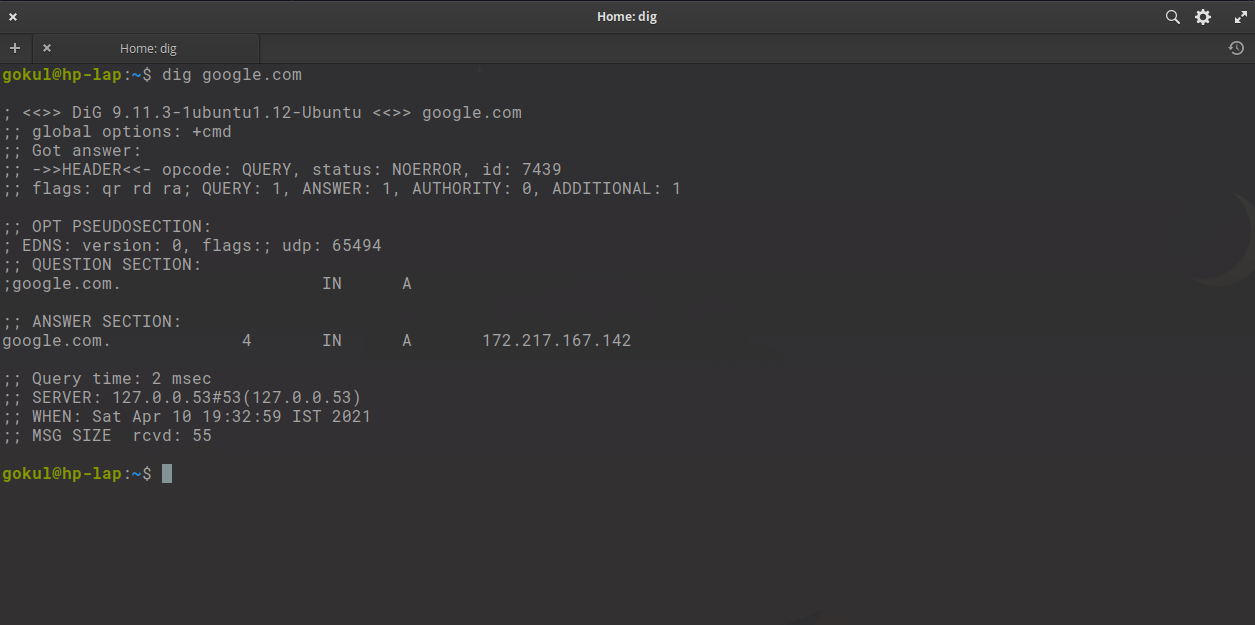
\includegraphics[width=0.90\textwidth]{img/p1/ss7.png}
\end{center}


\subsubsection{arp}
Arp manipulates or displays the kernel's IPv4 network neighbour cache. It can add entries to the table, delete one or
display the current content.
ARP stands for Address Resolution Protocol, which is used to find the media access control address of a network neighbour
for a given IPv4 Address.
\linebreak[2]

Syntax:
\begin{lstlisting}
arp [-vn] [-H type] [-i if] [-ae] [hostname]

arp [-v] [-i if] -d hostname [pub]
 
arp [-v] [-H type] [-i if] -s hostname hw_addr [temp]
 
arp [-v] [-H type] [-i if] -s hostname hw_addr [netmask nm] pub
 
arp [-v] [-H type] [-i if] -Ds hostname ifname [netmask nm] pub
 
arp [-vnD] [-H type] [-i if] -f [filename] 
\end{lstlisting}

\begin{center}
	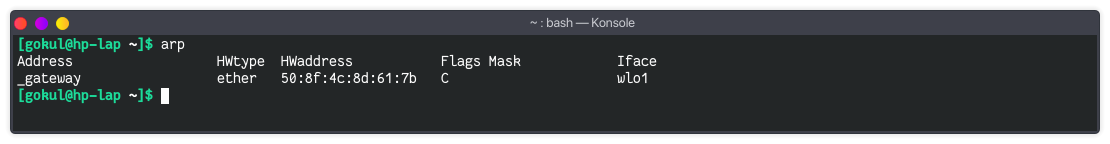
\includegraphics[width=0.90\textwidth]{img/p1/ss8.png}
\end{center}


\subsubsection{host}
host is a simple utility for performing DNS lookups. It is normally used to convert names to IP addresses and vice versa.
When no arguments or options are given, host prints a short summary of its command-line arguments and options.

name is the domain name that is to be looked up. It can also be a dotted-decimal IPv4 address or a colon-delimited IPv6
address, in which case host by default performs a reverse lookup for that address.  server is an optional argument  which
is  either  the  name  or IP address of the name server that host should query instead of the server or servers listed in
/etc/resolv.conf.
\linebreak[2]

Syntax:
\begin{lstlisting}
host  [-aACdlnrsTUwv] [-c class] [-N ndots] [-p port] [-R number] 
	[-t type] [-W wait] [-m flag] [ [-4] | [-6] ] [-v] [-V] 
	{name} [server]
\end{lstlisting}

\begin{center}
	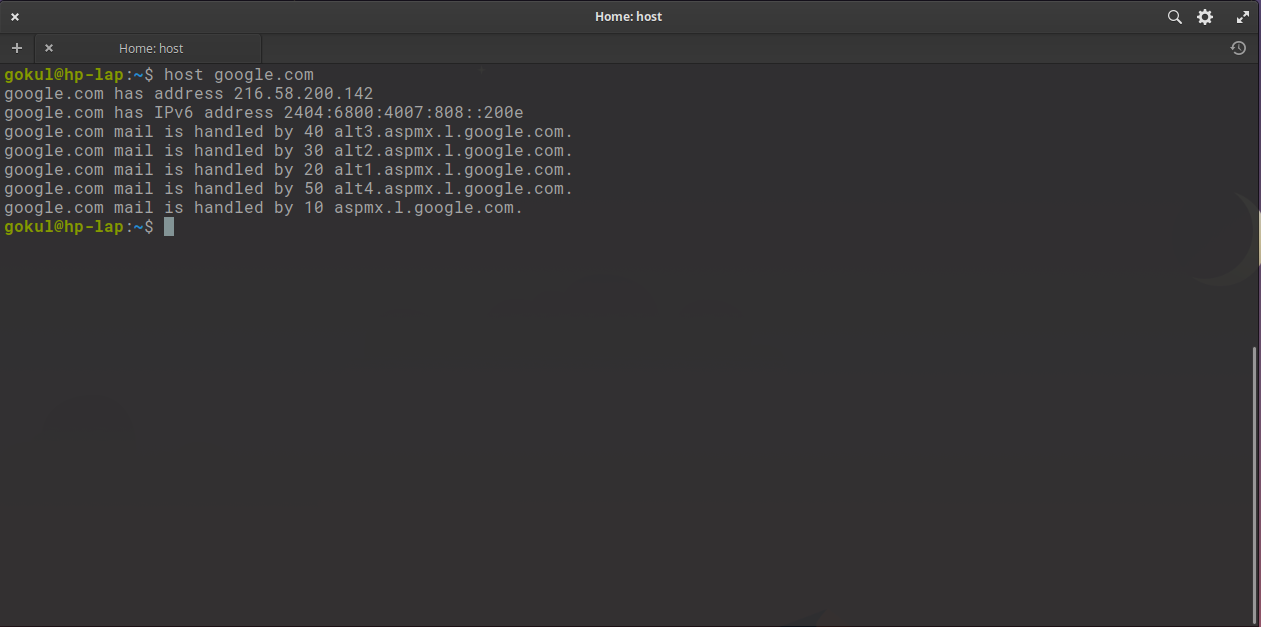
\includegraphics[width=0.90\textwidth]{img/p1/ss9.png}
\end{center}


\subsubsection{hostname}
Show or set the system's host name
\linebreak[2]

Syntax:
\begin{lstlisting}
hostname [OPTION...] [NAME]
\end{lstlisting}

\begin{center}
	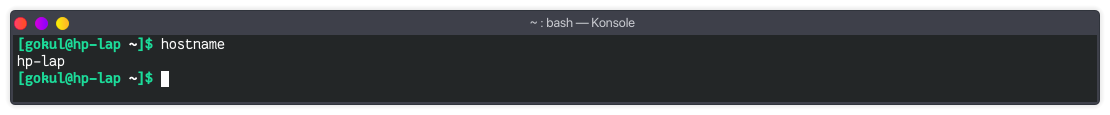
\includegraphics[width=0.90\textwidth]{img/p1/ss10.png}
\end{center}


\subsubsection{ethtool}
ethtool is used to query and control network device driver and hardware settings, particularly for wired Ethernet devices.
devname is the name of the network device on which ethtool should operate.
\linebreak[2]

Syntax:
\begin{lstlisting}
ethtool devname
\end{lstlisting}

\begin{center}
	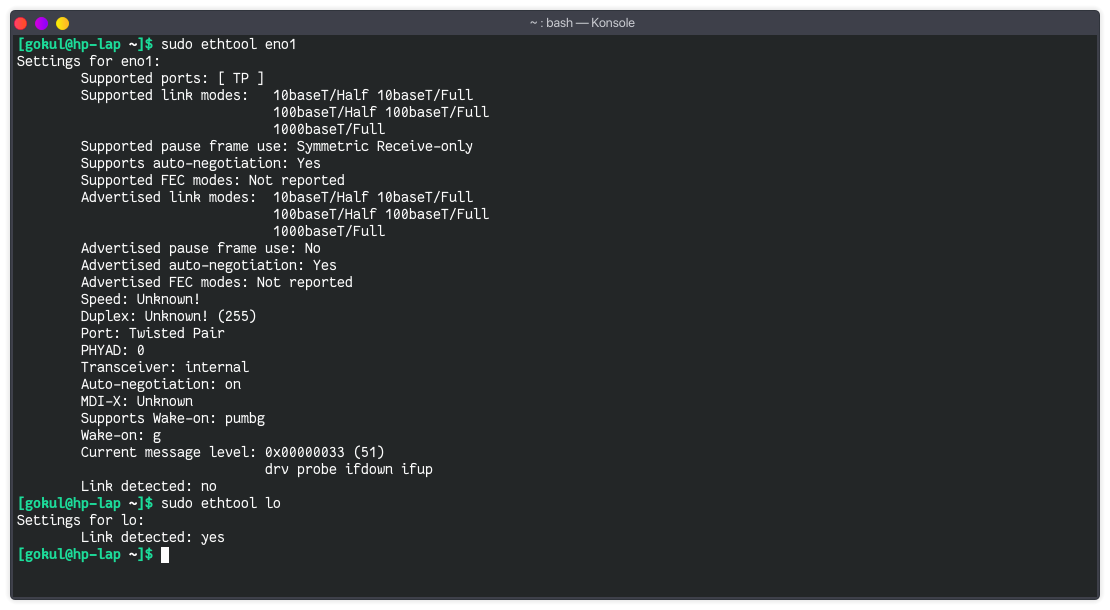
\includegraphics[width=0.90\textwidth]{img/p1/ss11.png}
\end{center}

\subsection{Result}
The above commands were executed and their outputs were verified